\section{Application}

\subsection{Traversing syntax trees to describe code}

We demonstrate an example of walking a syntax tree to generate a natural language description of a CSS selector in Figure~\ref{alg:css_traversal}.

\begin{figure}
\begin{algorithmic}

\Function{visit\_node}{node}
    \State clause = plural(node.element)
    \If{node has id}
        \State clause += (` with ID ' + node.id)
    \ElsIf{node has class}
        \State clause += (` of class ' + node.class)
    \EndIf
    \If{node has child}
        \State ch\_clause = visit\_node(node.child)
        \State clause = ch\_clause + `from' + clause
    \EndIf
    \State \Return clause
\EndFunction

\State
\Function{main}{parse\_tree}
    \State root\_clause = \Call{visit\_node}{parse\_tree.root}
    \State print ``This selector chooses '' + root\_clause
\EndFunction

\end{algorithmic}
\label{alg:css_traversal}
\caption{Procedure for generating text description of a CSS selector by traversing the parse tree.
\andrew{Note that a cheap shot here might be, how do we describe a node with both a class and ID?
The lame answer is that we currently don't.}
}
\end{figure}

\subsection{Mining and exposing hierarchy}

\begin{figure}
\centering{
    \framebox{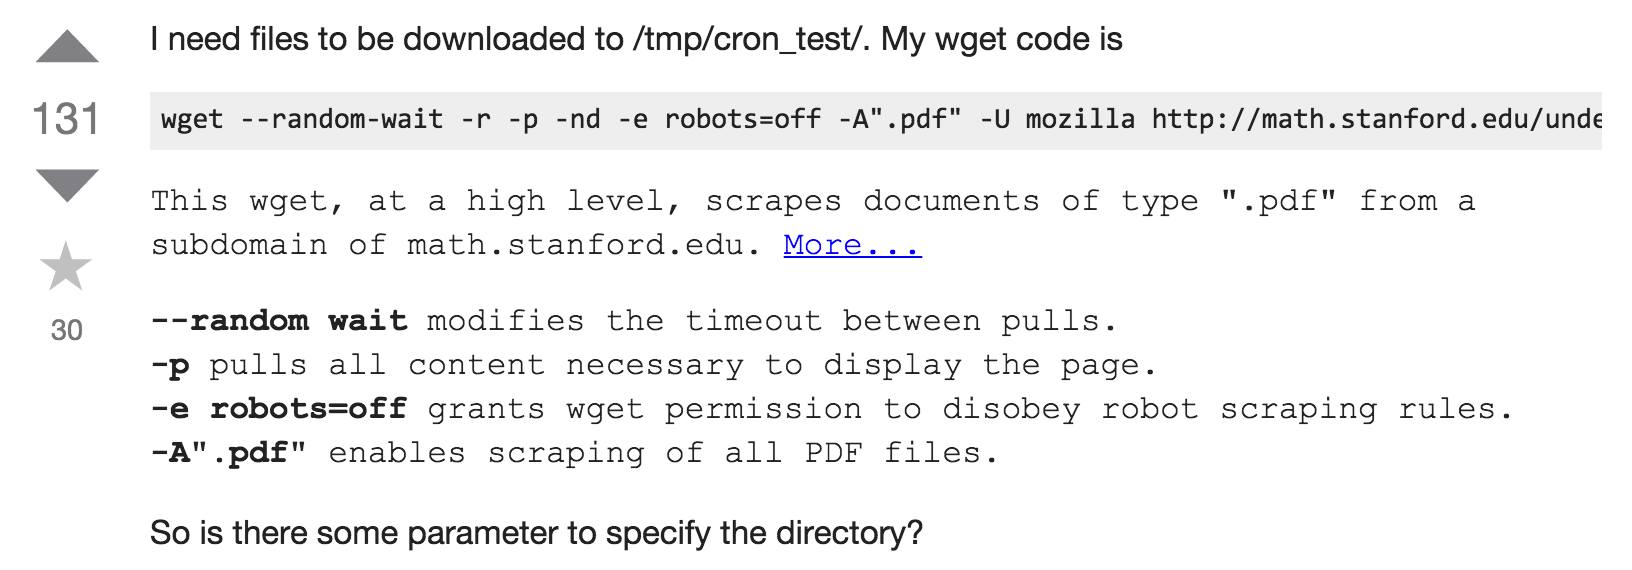
\includegraphics[width=.4\textwidth]{figures/so_wget_explanation}}
    \label{fig:so_wget_explanation}
    \caption{Expandable textual augmentation describing overview of command, followed by a fine-grained detailing of its arguments.}
}
\end{figure}

Using StackOverflow, developers can mine combinations of parameters that mean more than the sum of individual parameters.
For example, for \texttt{wget}, the combination of the \texttt{-r}, \texttt{-l<level>}, \texttt{-A<ext>}, and \texttt{-e robots=off} tags suggest that a user is about to scrape a destination URL recursively to depth level \texttt{l} for files of type \texttt{A}, without following the recommended etiquette for crawler \texttt{robots}.
\bjoern{This is really cool — does the technique apply generally to other types of tutorons?}
Through a preliminary effort with \texttt{wget}, we showed that one can find reasonable combinations of arguments that should be described together by scraping and observing frequent combinations of arguments from commands scraped from StackOverflow (Figure~\ref{fig:wget_arguments}).

Using this procedure, we can create explanations like those in (Figure~\ref{fig:so_wget_explanation}).
An initial description may just contain an overview of what the command does as a whole, inferred from the combination of arguments.
However, asking for information can provide a detailed breakdown of how each option affects the execution of the command.

\begin{figure}
\centering{
    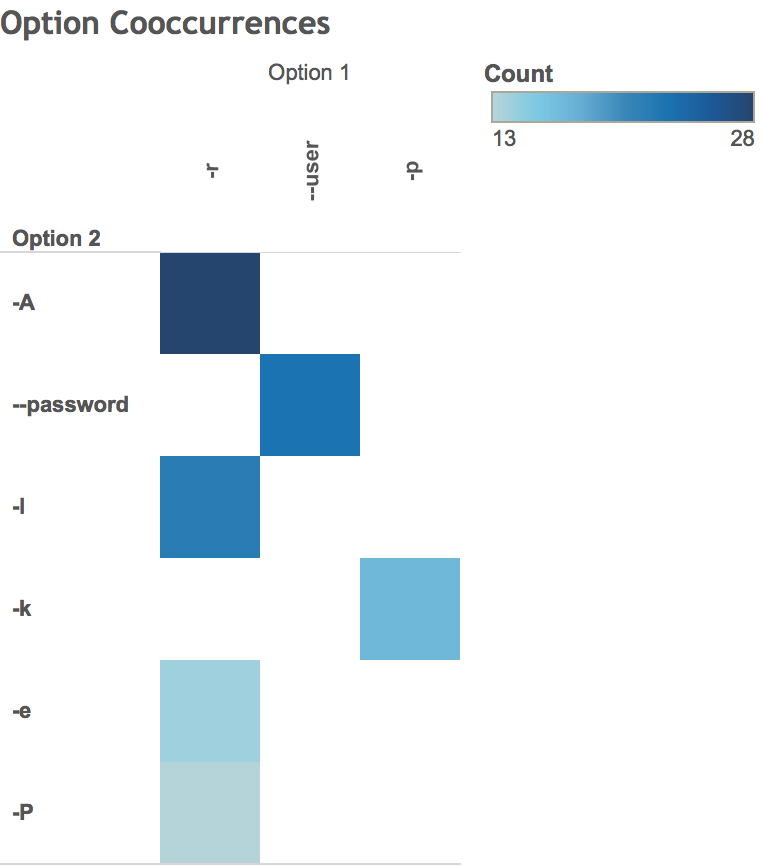
\includegraphics[width=.3\textwidth]{figures/wget_arguments}
}
\caption{\texttt{wget} arguments that frequently co-occur in uses of \texttt{wget} in StackOverflow questions. \andrew{A table would may be more readable here.}}
\label{fig:wget_arguments}
\end{figure}


\subsection{Generating examples}

\bjoern{Wait, there are so many different examples flying by right now.
Would all tutorons use the  techniques in sub-sections A-D here? Or each tutoron just one? I’m a bit confused about the higher-level argument.}
\bjoern{I think instead of showing a bunch of point examples that are all really  different from each other, we need to think about commonalities between them.
Otherwise reviewers may wonder why there’s a regular expression sub-project described here that doesn’t connect to other examples.}
We expect that similar approaches could be used to automically generate just-in-time exercises related to content of code in tutorials users are viewing. 
\andrew{Some reference to related work in exercise generation here would be appropriate.}

Long regular expressions are cryptic even for expert readers to understand.
We expect that in some contexts, providing readable examples of what strings will satisfy and fail to satisfy these patterns could help with comprehension of the regular expressions.

For the sake of showing that this concept would work, we determined guidelines for producing example strings that match a regular expression pattern.
Although there is an unbound number of strings that satisfy regular expressions that have repetitions, we want to limit the number of results to a readable, representative group.
We arbitrarily choose an ideal of 3-4 positive and 3-4 negative examples, though provide users the ability to request additional examples.

Cursorily, the process of generating relevant examples is as follows.
We start by producing an \emph{urtext}, a base version that satisfies the regular expression.
For each repeated group (not just a character) (* or +), we generate it exactly once to make sure that the group appears in the original best example.
We print any literal exactly as it appears in the pattern.
We choose on representative of each branch.
Whenever we have a repeated sequence of alphanumeric characters (repeated by + or *), we choose a dictionary word 5 letters in length and append 2 numbers.
If there are any symbols in the character class for this word, we choose a random sample of 2 of these symbols.
This forms our \emph{urtext}, which is the first positive example.

We view each regular expression as a graph of \emph{branches}, \emph{choices}, \emph{repetitions}, and \emph{literals}.
To create an alternative correct answer, we perform each just one operation to one node on top of the urtext:
\begin{itemize}
\item Flip a branch to choose a different child
\item Choose an alternative dictionary word and sampling of numbers and symbols for word choices
\item For + repetitions, toggle 1 repetition to 2.  For * repetitions, toggle 1 repetition to 0.
\end{itemize}

We generate alternative correct answers by performing one operation at each node, holding the rest of the tree at its urtext form.
We suspect that altering only one part of the string while holding the rest constant will improve reader's ability to detect what change is acceptable for the string to satisfy the pattern.
We choose the urtext and randomly sample 3 valid alternatives for the correct examples of a regular expression.
Similarly, we alter one character or repetition at a time for each node to generate failure cases.

In the future, we would like to implement in-place editors of regular expressions that enables real-time updating of these examples and checking user-defined test patterns.

\subsection{Chaining \glspl{name} to describe each other}

\andrew{This needs to be contextualized.}
To demonstrate that \glspl{name} can be used together, we developed a \gls{name} that is capable of explaining HTML elements.
This can be applied to explanations generated by the CSS \gls{name}.
In this way, an ecosystem of complementary descriptions can help shed light on a larger, unfamiliar space like general web development.

\section{Applications}

\subsection{Providing Fine-Grained Tutorial Clarifications}

\subsection{Code Comprehension}

\subsection{Helping Authors Fill In New Tutorials}

This use case is highly experimental, but can technically be done.
See an example of early text of a tutorial explaining building up CSS selectors (Figure~\ref{fig:tutorial_generation}).
One advantage of this model is avoiding the rote descriptions that one would have to make, and even looking up API or language specifics to make sure that your tutorial is factually correct, as you start with a developer-provided ground truth of what the grammar does.

\begin{figure}
\centering{
    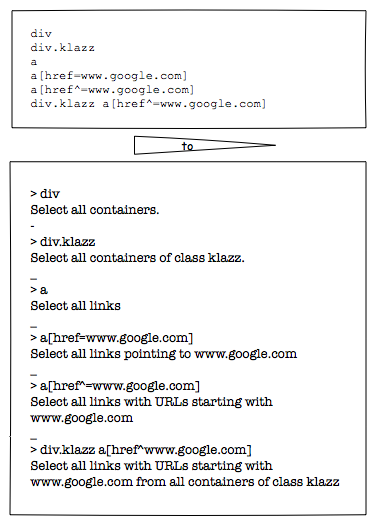
\includegraphics[width=.4\textwidth]{figures/tutorial_generation}
}
\caption{The building blocks of a tutorial on CSS selectors, auto-generated by a \gls{name}.}
% \label{fig:tutorial_generation}
\end{figure}
